%%%%%%%%%%%%%%%%%%%%%%%%%%%%%%%%%%%%%%%%%%%%%%%%%%%%%%%%%%%%%%%%%%%%%%%%%%%%%%%%%%%
%% This project aims to create  a custom  UDL template for presentation.                %%
%% author: BOUKLI HACENE Sofiane - Prof in Computer Science Departement (UDL)   %%
%% contacts:                                                                     %%
%%    e-mail: boukli@univ-sba.dz                                                   %%

%%%%%%%%%%%%%%%%%%%%%%%%%%%%%%%%%%%%%%%%%%%%%%%%%%%%%%%%%%%%%%%%%%%%%%%%%%%%%%%%%%%

\documentclass{libs/udl_format}
% Inserting the preamble file with the packages
\input{libs/preamble.tex}
% Inserting the references file
\bibliography{references.bib}

% Title
\title[Roteamento Dinâmico de Consultas SQL]{\huge\textbf{Roteamento Dinâmico de Consultas SQL}}
% Subtitle
\subtitle{Baseado em Metadados de Tabelas Apache Iceberg}
% Author of the presentation
\author{Aristides Henrique Gonçalves da Cruz}
% Institute's Name
\institute[PUCMinas]{
% email for contact
    \normalsize{\email{arihenriquedev@hotmail.com}}
    \speciality{Sistemas de Informação}
    \department{ICEI}
    PUCMinas São Gabriel
}
% date of the presentation
\date{Novembro de 2025}

%%%%%%%%%%%%%%%%%%%%%%%%%%%%%%%%%%%%%%%%%%%%%%%%%%%%%%%%%%%%%%%%%%%%%%%%%%%%%%%%%%
%% Start Document of the Presentation                                           %%               
%%%%%%%%%%%%%%%%%%%%%%%%%%%%%%%%%%%%%%%%%%%%%%%%%%%%%%%%%%%%%%%%%%%%%%%%%%%%%%%%%%
\begin{document}
% insert the code style
    \input{libs/code_style}

% Slide 1: Capa
    \begin{frame}{}
        \centering{\calligra{Entrega Final}}
        \maketitle

        \hspace{1.5cm}  {
            \resizebox{0.8\textwidth}{!}{
                \begin{tabular}{llll}
                    \textbf{Trabalho:}  & \textsc{Trabalho de Conclusão de Curso} & & \\
                    \textbf{Curso:}  & \textsc{Sistemas de Informação} & & \\
                    \textbf{Instituição:}  & \textsc{PUC Minas - Unidade São Gabriel} & & \\
                \end{tabular}
            }
        }

        \normalsize
    \end{frame}

% Slide 2: Estrutura da apresentação
    \begin{frame}{Estrutura da Apresentação}
        \begin{enumerate}
            \item \textbf{Objetivos e Justificativa}
            \begin{itemize}
                \item Objetivo Geral
                \item Objetivos Específicos
                \item Justificativa
            \end{itemize}
            \vspace{0.3cm}
            \item \textbf{Metodologia}
            \begin{itemize}
                \item Arquitetura (Diagramas C4)
                \item Algoritmo de Decisão
            \end{itemize}
            \vspace{0.3cm}
            \item \textbf{Expectativas e Resultados}
            \vspace{0.3cm}
            \item \textbf{Conclusão}
        \end{enumerate}
    \end{frame}

% Slide 3: Objetivo Geral
    \begin{frame}{Objetivo Geral}
        \begin{alertblock}{}
            Desenvolver o \textit{DyraSQL}, um mecanismo de decisão que utiliza metadados de tabelas \textit{Apache Iceberg} através do comando \textit{EXPLAIN (TYPE IO)} do \textit{Trino} para definir automaticamente o \textit{cluster} mais adequado para execução de consultas SQL.
        \end{alertblock}
        
        \vspace{0.5cm}
        \begin{block}{Problema}
            Escolha estática de \textit{clusters} \textit{Trino} (leve versus robusto) sem considerar características dos dados e complexidade das consultas.
        \end{block}
    \end{frame}

% Slide 4: Objetivos Específicos
    \begin{frame}{Objetivos Específicos}
        \begin{enumerate}
            \item Mapear e caracterizar os metadados disponíveis em tabelas \textit{Apache Iceberg}, identificando indicadores de volume de dados, complexidade da query e custo esperado de execução.
            \vspace{0.2cm}
            \item Estabelecer regras de decisão para roteamento de consultas, classificando-as em \textit{clusters} leve, intermediário e robusto.
            \vspace{0.2cm}
            \item Projetar e desenvolver um protótipo funcional do \textit{DyraSQL} em ambiente local, utilizando o \textit{Trino}, Docker Compose, MinIO e PostgreSQL.
            \vspace{0.2cm}
            \item Realizar experimentos controlados em cenários distintos de carga de trabalho, verificando a viabilidade técnica e coletando métricas de tempo de execução, consumo de recursos e custo associado.
        \end{enumerate}
    \end{frame}

% Slide 5: Justificativa
    \begin{frame}{Justificativa}
        \begin{block}{Necessidade}
            \begin{itemize}
                \item Crescimento do volume de dados em \textit{data lakes}
                \item Necessidade de equilibrar custos e desempenho na execução de consultas SQL
                \item Escolha estática de \textit{clusters} \textit{Trino} resulta em provisionamento excessivo ou subdimensionamento
            \end{itemize}
        \end{block}
        
        \vspace{0.3cm}
        \begin{alertblock}{Impacto Esperado}
            Melhor custo-benefício e utilização eficiente de recursos através de roteamento baseado em análise prévia de metadados.
        \end{alertblock}
    \end{frame}

% Slide 6: Revisão Bibliográfica - Fundamentos
    \begin{frame}{Revisão Bibliográfica - Fundamentos}
        \begin{block}{Fundamentos Teóricos}
            \begin{itemize}
                \item \textbf{\textit{Apache Iceberg}:} Formato de tabela que oferece metadados hierárquicos para gestão eficiente de dados em \textit{data lakes}
                \item \textbf{\textit{Trino}:} \textit{Engine} de consultas distribuído que suporta \textit{EXPLAIN (TYPE IO)} para análise prévia de custos
                \item \textbf{Metadados para melhoria:} Informações sobre volume de dados, partições e filtros podem ser utilizadas para estimativa de custo de execução
            \end{itemize}
        \end{block}
        
        \vspace{0.2cm}
        \begin{exampleblock}{Aproveitamento}
            O \textit{DyraSQL} utiliza o \textit{EXPLAIN (TYPE IO)} do \textit{Trino} para extrair metadados precisos sobre volume efetivo de dados antes da execução.
        \end{exampleblock}
    \end{frame}

% Slide 7: Revisão Bibliográfica - Trabalhos Relacionados
    \begin{frame}{Revisão Bibliográfica - Trabalhos Relacionados}
        \begin{block}{Trabalhos Principais}
            \begin{itemize}
                \item \textbf{Xue et al. (2024):} Sistema adaptativo para execução de consultas em \textit{lakehouse} em larga escala
                \item \textbf{Strausz et al. (2025):} Otimizador baseado em modelo de custo aprendido para \textit{workloads} SQL \textit{multi-engine}
                \item \textbf{Weintraub et al. (2024):} Otimização de consultas em \textit{data lakes} baseada em planos de cobertura balanceados
            \end{itemize}
        \end{block}
        
        \vspace{0.2cm}
        \begin{alertblock}{Diferenciação}
            O \textit{DyraSQL} propõe roteamento entre \textit{clusters} \textit{Trino} de capacidades distintas (leve, intermediário e robusto) baseado em análise prévia de metadados do \textit{Apache Iceberg}.
        \end{alertblock}
    \end{frame}

% Slide 8: Metodologia
    \begin{frame}{Metodologia}
        \begin{enumerate}
            \item \textbf{Extração de Metadados}
            \begin{itemize}
                \item Utilização do \textit{EXPLAIN (TYPE IO)} do \textit{Trino}
                \item Extração de \textit{outputSizeInBytes}, \textit{outputRowCount}, \textit{cpuCost}
            \end{itemize}
            \vspace{0.2cm}
            \item \textbf{Algoritmo de Decisão}
            \begin{itemize}
                \item Cálculo de \textit{Score} baseado em três fatores: volume, complexidade e histórico
                \item Direcionamento para leve (Score < 0,3), intermediário (0,3-0,7) ou robusto (> 0,7)
            \end{itemize}
            \vspace{0.2cm}
            \item \textbf{Implementação}
            \begin{itemize}
                \item \textit{Trino Gateway Proxy} para interceptação de consultas
                \item \textit{DyraSQL Core} para análise e decisão de roteamento
                \item Integração com PostgreSQL para histórico e \textit{cache}
            \end{itemize}
        \end{enumerate}
    \end{frame}

% Slide 9: Continuação da Metodologia - Contexto
    \begin{frame}{Metodologia - Contexto do Sistema}
        \vspace{-0.6cm}
        \begin{center}
            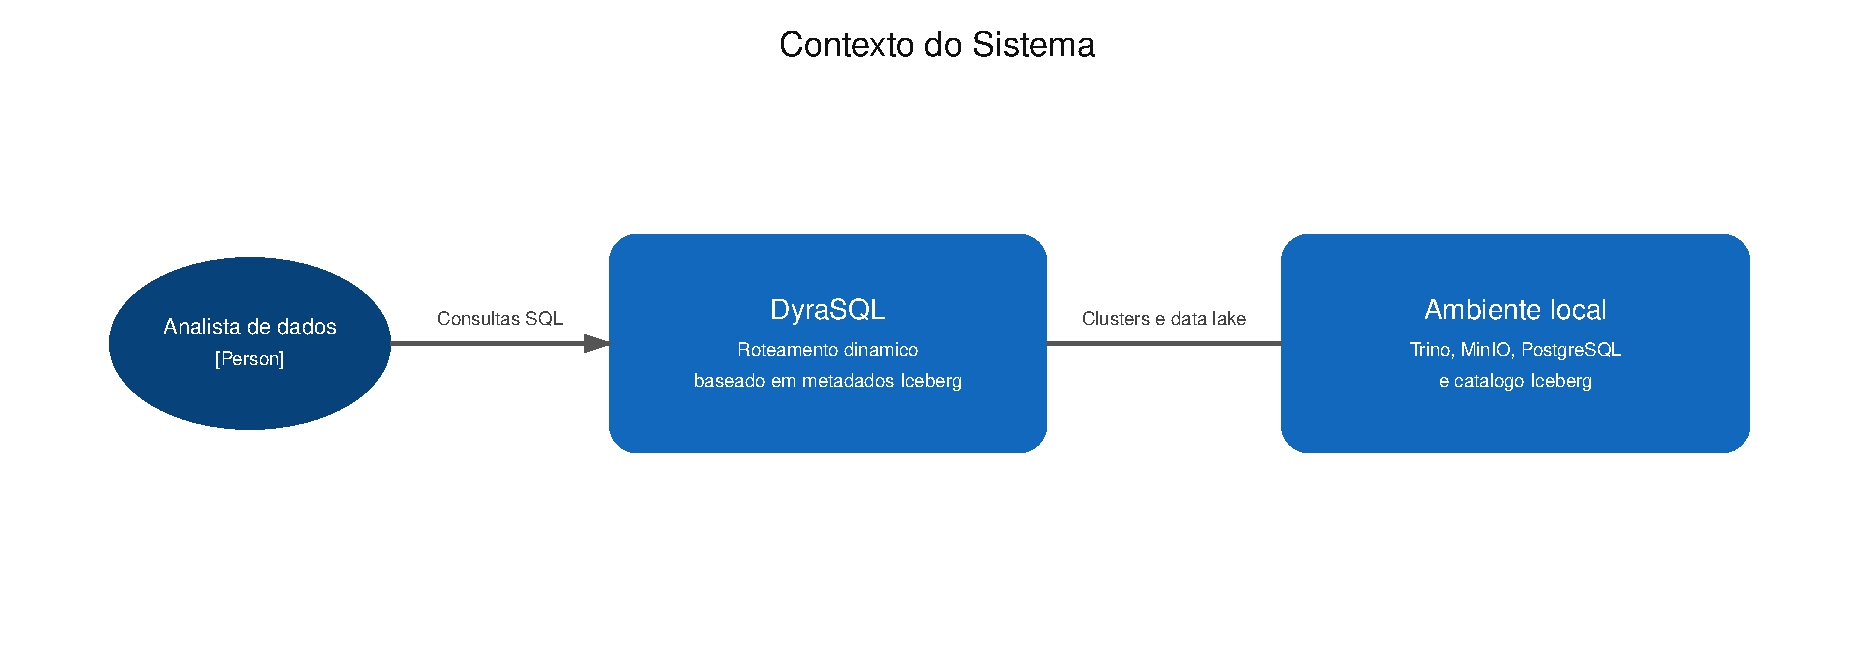
\includegraphics[width=0.95\textwidth,height=0.55\textheight,keepaspectratio]{../figuras/c4_1.pdf}
        \end{center}
        \vspace{0.05cm}
        \tiny{\textcolor{blue_theme}{\textbf{Fonte:}} Elaborado pelo autor.}
    \end{frame}

% Slide 10: Continuação da Metodologia - Containers
    \begin{frame}{Metodologia - Containers do Sistema}
        \vspace{-0.3cm}
        \begin{center}
            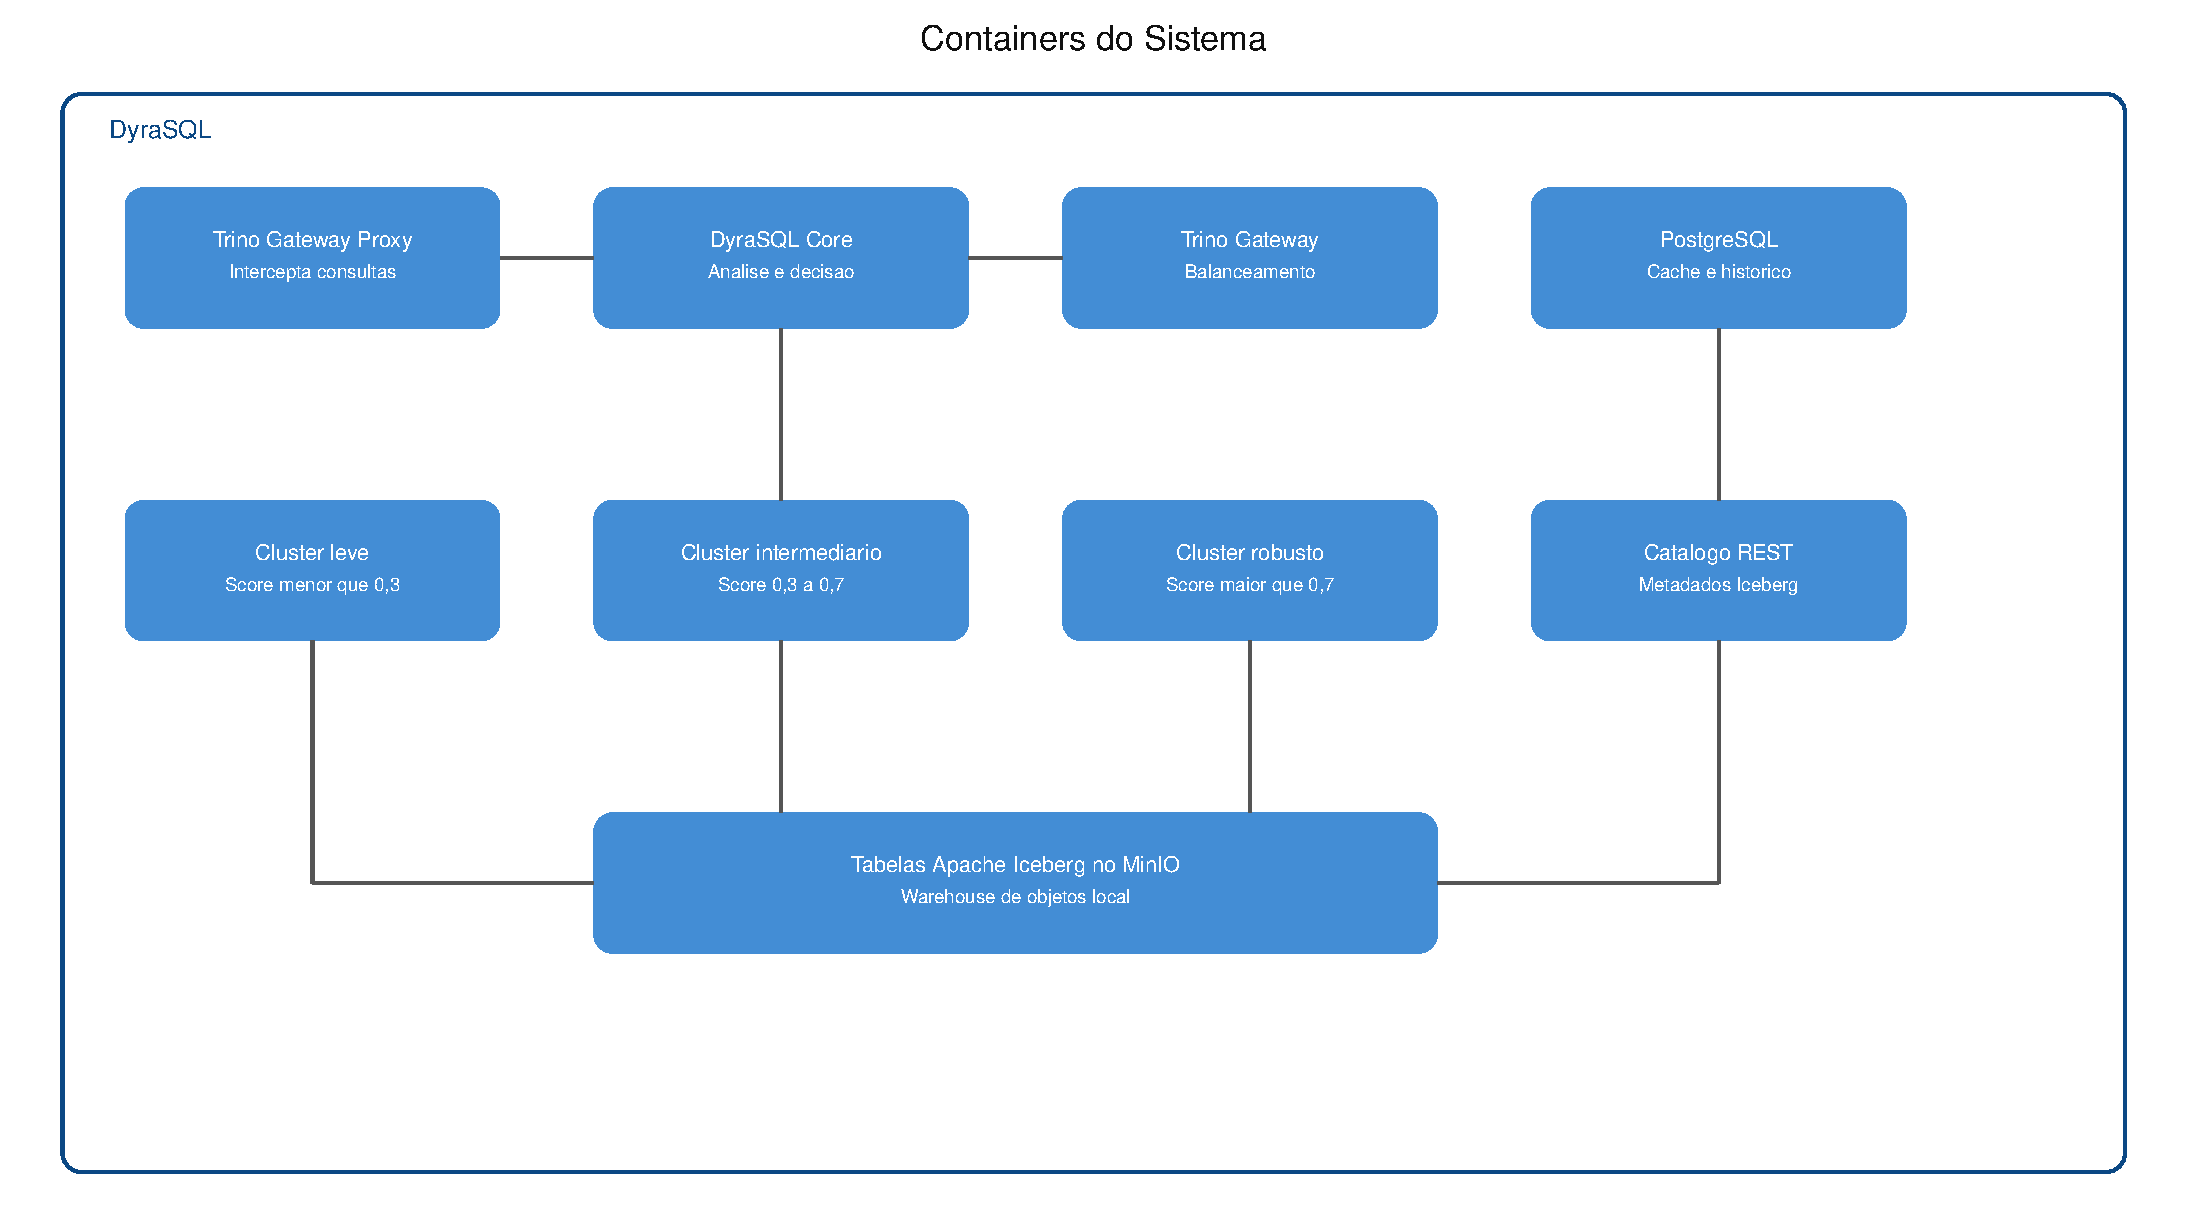
\includegraphics[width=0.95\textwidth,height=0.65\textheight,keepaspectratio]{../figuras/c4_2.pdf}
        \end{center}
        \vspace{0.1cm}
        \tiny{\textcolor{blue_theme}{\textbf{Componentes:}} Trino Gateway Proxy, Trino Gateway, DyraSQL Core, Clusters de Execução}
    \end{frame}

% Slide 11: Continuação da Metodologia - Componentes
    \begin{frame}{Metodologia - Componentes Internos}
        \vspace{-0.3cm}
        \begin{center}
            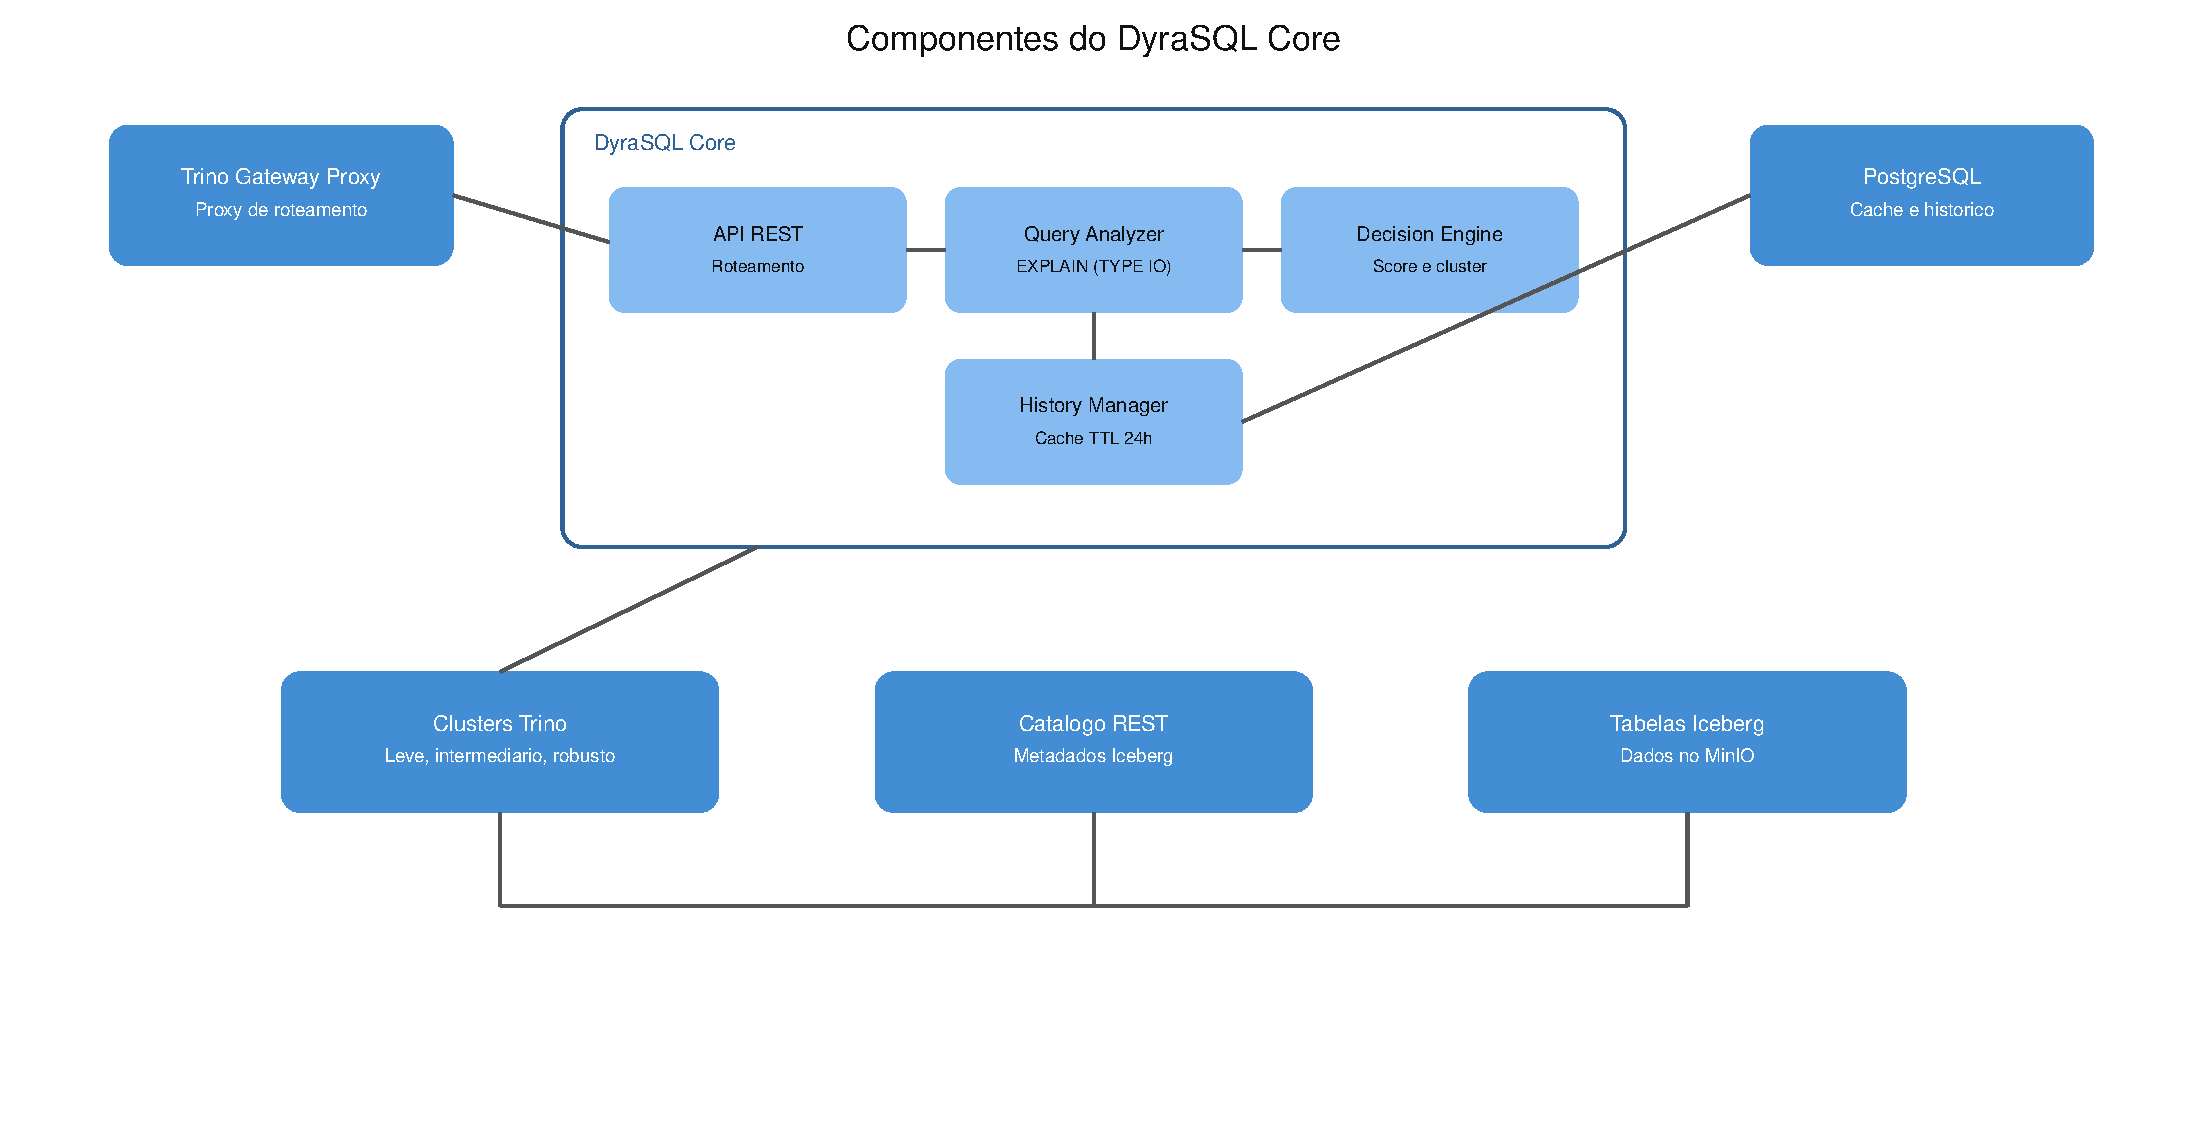
\includegraphics[width=0.95\textwidth,height=0.65\textheight,keepaspectratio]{../figuras/c4_3.pdf}
        \end{center}
        \vspace{0.1cm}
        \tiny{\textcolor{blue_theme}{\textbf{Fluxo:}} Interceptação → Análise → Decisão → Execução → Feedback}
    \end{frame}

% Slide 12: Continuação da Metodologia - Algoritmo
    \begin{frame}{Metodologia - Algoritmo de Decisão}
        \begin{block}{Fórmula de Pontuação}
            \begin{equation}
                S = w_1 \times f_v + w_2 \times f_c + w_3 \times f_h
            \end{equation}
            \begin{itemize}
                \item $f_v$: Fator de volume (50\%)
                \item $f_c$: Fator de complexidade (30\%)
                \item $f_h$: Fator histórico (20\%)
            \end{itemize}
        \end{block}
        
        \vspace{0.3cm}
        \begin{alertblock}{Decisão de Roteamento}
            \begin{itemize}
                \item Score $< 0,3$: \textit{cluster} leve
                \item Score $0,3-0,7$: \textit{cluster} intermediário
                \item Score $> 0,7$: \textit{cluster} robusto
            \end{itemize}
        \end{alertblock}
    \end{frame}

% Slide 13: Configurações dos Ambientes
    \begin{frame}{Metodologia - Configurações dos Ambientes}
        \begin{block}{\textit{cluster} leve (Score $< 0,3$)}
            \begin{itemize}
                \item \textbf{Memória:} 2 GB de heap
                \item \textbf{Memória máxima por query:} 1 GB
                \item \textbf{Tempo máximo de execução:} 5 minutos
                \item \textbf{Uso:} Consultas leves
            \end{itemize}
        \end{block}

        \begin{block}{\textit{cluster} intermediário (Score $0,3-0,7$)}
            \begin{itemize}
                \item \textbf{Memória:} 3 GB de heap
                \item \textbf{Memória máxima por query:} 2 GB
                \item \textbf{Tempo máximo de execução:} 15 minutos
                \item \textbf{Uso:} Consultas intermediárias
            \end{itemize}
        \end{block}
    \end{frame}

    \begin{frame}{Metodologia - Configurações dos Ambientes (continuação)}
        \begin{block}{\textit{cluster} robusto (Score $> 0,7$)}
            \begin{itemize}
                \item \textbf{Memória:} 4 GB de heap
                \item \textbf{Memória máxima por query:} 3 GB
                \item \textbf{Tempo máximo de execução:} 30 minutos
                \item \textbf{Uso:} Consultas pesadas
            \end{itemize}
        \end{block}

        \vspace{0.3cm}
        \begin{alertblock}{Configuração compartilhada}
            \begin{itemize}
                \item Catálogo \textit{Iceberg} REST
                \item MinIO para armazenamento de objetos
                \item Acesso unificado às tabelas independentemente do \textit{cluster}
            \end{itemize}
        \end{alertblock}
    \end{frame}

% Slide 15: Expectativas

% Slide 15: Expectativas
    \begin{frame}{Expectativas}
        \begin{block}{Resultados Esperados}
            \begin{itemize}
                \item \textbf{Precisão:} Sistema capaz de calcular \textit{scores} precisos e direcionar consultas para os \textit{clusters} apropriados
                \item \textbf{Eficiência:} Tempo de análise prévia inferior a 200ms
                \item \textbf{Consistência:} Consultas similares recebem \textit{scores} próximos e são direcionadas para os mesmos tipos de \textit{clusters}
                \item \textbf{Melhoria de Custo-Benefício:} Redução de custos operacionais através de roteamento inteligente
            \end{itemize}
        \end{block}
    \end{frame}

% Slide 16: Resultados
    \begin{frame}{Resultados}
        \begin{block}{Experimentos Realizados}
            \begin{itemize}
                \item Dataset sintético em tabelas \textit{Apache Iceberg} no MinIO
                \item Consultas variadas: diferentes volumes, complexidades e estruturas
                \item Métricas coletadas: precisão dos \textit{scores}, adequação das decisões, eficiência do sistema
            \end{itemize}
        \end{block}
        
        \vspace{0.3cm}
        \begin{alertblock}{Principais Resultados}
            \begin{itemize}
                \item Extração de metadados eficiente: tempo médio < 200ms
                \item \textit{Scores} precisos e consistentes para consultas similares
                \item Diferenciação adequada entre consultas leves, intermediárias e pesadas
            \end{itemize}
        \end{alertblock}
    \end{frame}

% Slide 17: Desafios da Pesquisa
    \begin{frame}{Desafios da Pesquisa}
        \begin{block}{Desafios Identificados}
            \begin{itemize}
                \item \textbf{Dependência de Histórico:} Precisão das decisões depende de histórico suficiente no PostgreSQL
                \item \textbf{Limitações do EXPLAIN:} Consultas muito complexas podem exceder 500ms de análise
                \item \textbf{Qualidade dos Metadados:} Dependência da qualidade e atualização dos metadados do \textit{Apache Iceberg}
                \item \textbf{Consultas Atípicas:} Consultas com características não previstas podem resultar em decisões subótimas
            \end{itemize}
        \end{block}
        
        \vspace{0.2cm}
        \begin{alertblock}{Mitigações}
            Sistema de \textit{cache} temporal, valores \textit{default} para casos sem histórico e aprendizado contínuo baseado em \textit{feedback}.
        \end{alertblock}
    \end{frame}

% Slide 18: Obrigado
    \begin{frame}{}
        \centering
        \vspace{2cm}
        {\huge \calligra{Obrigado!}}
        \vspace{1cm}
        \begin{block}{}
            \centering
            \textbf{Dúvidas?}
        \end{block}
    \end{frame}

\end{document}
